%!TEX root = Slic3r-Manual.tex
\section{Working with Models}

Yet another step lies between now and the first print - a model has to found and then sliced.

\subsection{Model Formats} % (fold)
\label{sub:model_formats}

Slic3r accepts the following file types.

\begin{itemize}
	\item STereoLithography (STL) files can come from a wide variety of sources and are now a de facto standard in 3D printing.  The files simply describe the surface geometry of a 3D object without any additional information (such as colour or material), and it is this simplicity that has probably made the format ubiquitous.
	\item Wavefront OBJ files are an open format originally used in an animation application from Wavefront Technologies, but has since been adopted by the wider 3D modelling community.  It is similar to the STL format.
	\item Additive Manufacturing File Format (AMF) was developed in response to the limited nature of the STL format.  In addition to describing the geometry of the 3D model it can also describe colours and materials, as well as more complex attributes, such as gradient mixes and multiple object arrangements (constellations).  Whilst the format is deemed a standard it has yet to be widely adopted in the 3D maker community.
\end{itemize}
% subsection model_formats (end)

\subsection{Finding Models} % (fold)
\label{sub:working_with_models}
The 3D model files may come from an online repository, such as Thingiverse\footnote{http://www.thingiverse.com} or GrabCAD\footnote{http://grabcad.com} or be created from a CAD program, such as FreeCAD\footnote{http://sourceforge.net/projects/free-cad}, Sketchup\footnote{http://www.sketchup.com}, or OpenSCAD\footnote{http://www.openscad.org}, or an online CAD tool such as Shapesmith\footnote{http://shapesmith.net}.  

You may wish to view the files before slicing and there are many free applications available, one of which is Meshlab\footnote{http://www.meshlab.org} - a comprehensive tool for viewing and working with 3D files.

\begin{figure}[H]
\centering
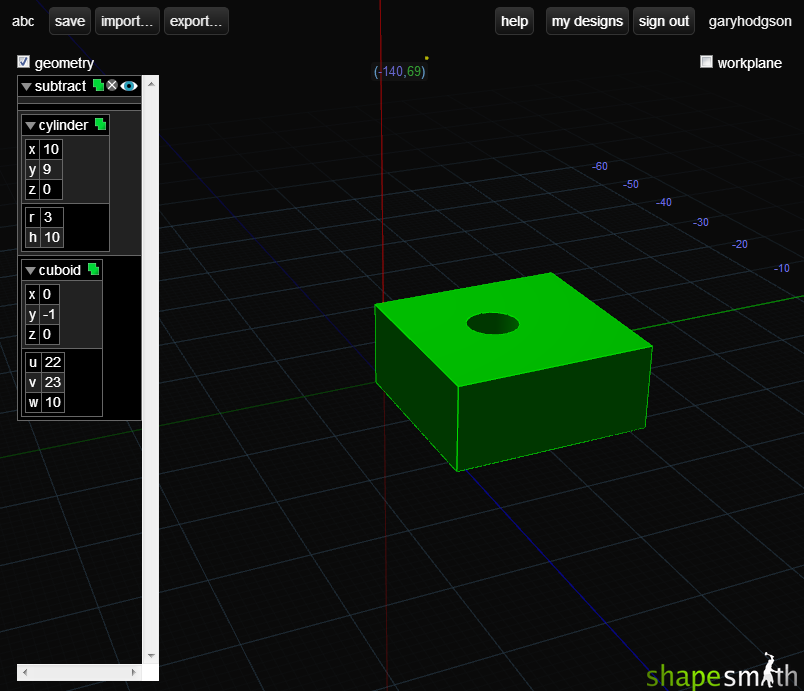
\includegraphics[keepaspectratio=true,width=0.75\textwidth]{working_with_models/shapesmith.png}
\caption{Shapesmith online CAD tool.}
\label{fig:shapesmith}
\end{figure}

% subsection working_with_models (end)


\subsection{Working with Plater} % (fold)
\label{sub:working_with_plater}
Slic3r has a tool, called Plater, which allows one or more models to be loaded and arranged before being sliced.

\begin{figure}[H]
\centering
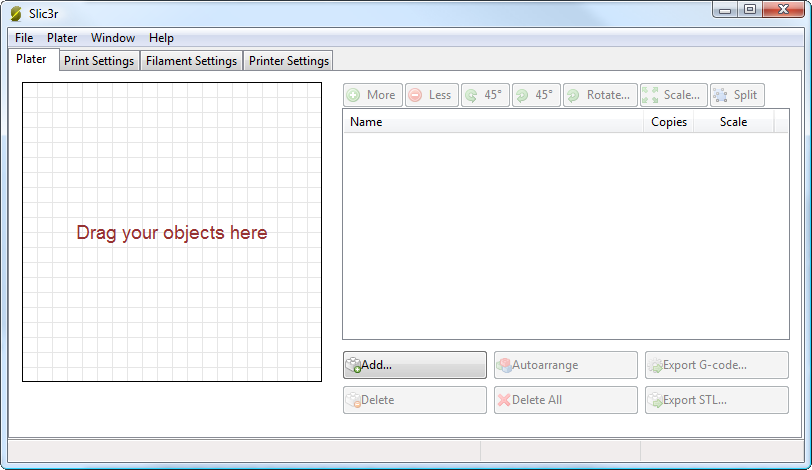
\includegraphics[keepaspectratio=true,width=0.75\textwidth]{working_with_models/plater.png}
\caption{Plater}
\label{fig:plater}
\end{figure}

Once you have acquired a model, drag it onto the Plater window (or use the Add button below the file list) to load it into Slic3r.  In the figure below, the traditional RepRap Minimug\footnote{http://www.thingiverse.com/thing:18357} is loaded, and is viewed from above. The ring around the model is a skirt - a single perimeter, several millimeters away from the model, which is extruded first.  This is useful in making sure the plastic is flowing smoothly from the nozzle when the model is starting to be printed.

\begin{figure}[H]
\centering
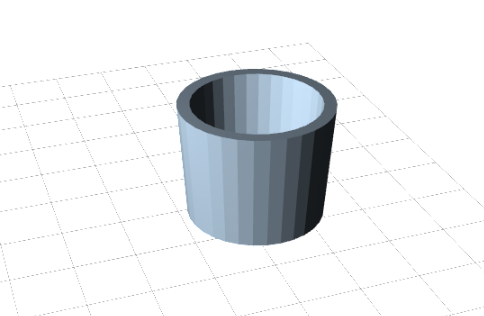
\includegraphics[keepaspectratio=true,width=0.75\textwidth]{working_with_models/minimug_model.png}
\caption{Minimug model.}
\label{fig:minimug_model}
\end{figure}

\begin{figure}[H]
\centering
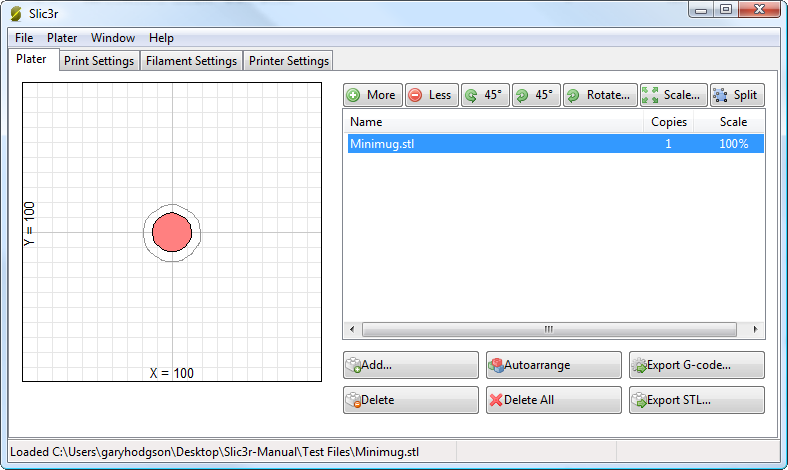
\includegraphics[keepaspectratio=true,width=0.75\textwidth]{working_with_models/plater_model_loaded.png}
\caption{STL file loaded.}
\label{fig:plater_model_loaded}
\end{figure}

The model can be repositioned by dragging the representation of it on the left of the screen around the bed.  Note that the dimensions of the bed should match your printer, as given during the initial configuration above.

On the right-hand side is the list of currently loaded files.  The buttons along the top of the file list allow you to arrange the models.
\begin{itemize}
	\item \textbf{More/Less}  - Adjust how many copies should be printed.
	\item \textbf{45°/Rotate}  - Rotate the selected model around the Z axis, either in 45° increments clockwise or counter-clockwise, or by a given amount.
	\item \textbf{Scale}  - Increase or decrease the size of the printed model.
	\item \textbf{Split}  - Divides a model which consists of more than one part into it's constituent parts, allowing each one to be arranged individually.
\end{itemize}

The buttons along the bottom of the file list allow you to add, remove, auto-arrange, or export the models.
\begin{itemize}
	\item \textbf{Add}  - Opens a file dialog to add a model to the plater, as an alternative to dropping a file directly.
	\item \textbf{Delete/Delete All}  - Remove one or all models from the plater.
	\item \textbf{Autoarrange}  - Attempt to arrange the models to give the optimal layout.
	\item \textbf{Export G-code}  - Starts slicing the model and produces a G-Code file.
	\item \textbf{Export STL}  - Save the current set of models as a single STL file.
\end{itemize}


% subsection working_with_plater (end)

\subsection{Cleaning STLs} % (fold)
\label{sub:cleaning_stls}
If the 3D mesh described in the model contains holes, or edges are misaligned (known as being non-manifold), then Slic3r may have problems working on it.  Slic3r will attempt to fix any problems it can, but some problems are out of it's reach.  If the application complains that a model cannot be sliced correctly then there are several options available, and the ones described here are all free at the time of writing. 

%%% CONFIGURATION TUNING %%%
{%!TEX root = Slic3r-Manual.tex

\paragraph{Netfabb Studio} % (fold)
\label{par:netfabb_studio}
Netfabb produce a range of 3D modelling applications, including a free basic version\footnote{http://www.netfabb.com/basic.php}.  This version includes a mesh repair module which can help eliminate the various problems faced.  Up-to-date instructions can be found on the Netfabb wiki\footnote{http://wiki.netfabb.com/Part\_Repair}, the following is a quick overview of the steps involved.

\begin{figure}[H]
\centering
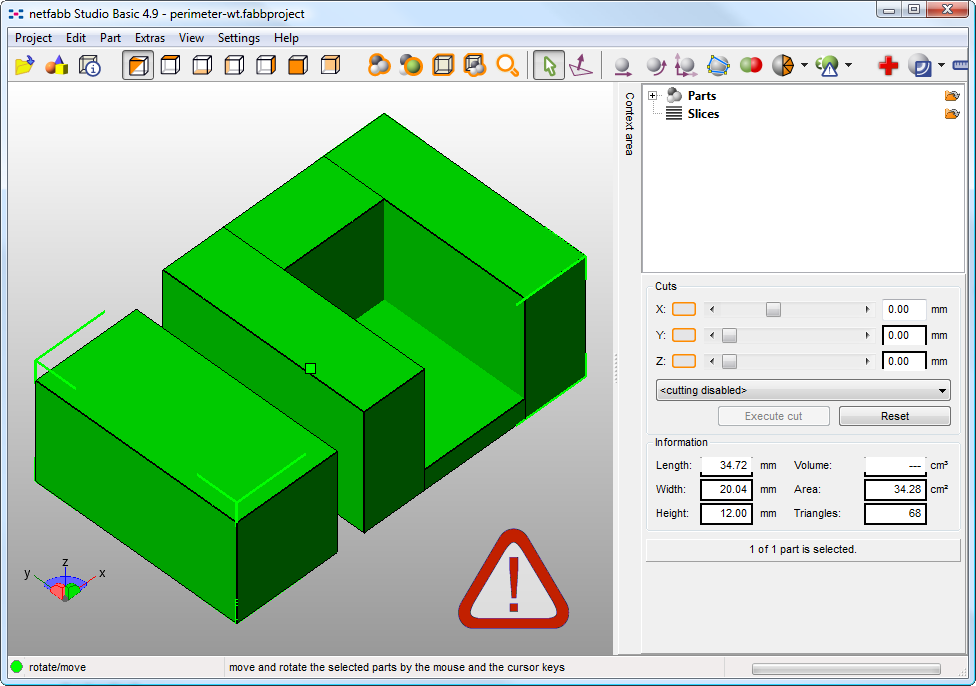
\includegraphics[keepaspectratio=true,width=0.75\textwidth]{working_with_models/netfabb_studio_part_repair.png}
\caption{Netfabb Studio: Part repair.}
\label{fig:netfabb_studio_part_repair}
\end{figure}

\begin{itemize}
	\item Start Netfabb Studio, and load the problem STL file, either via the \texttt{File} menu or by dragging and dropping it onto the workspace. If Netfabb detects a problem it will show a red warning sign in the bottom right-hand corner.
	\item To run the repair scripts, select the part and then either click the first aid icon in the toolbar (the red cross), or select from the context menu \texttt{Extras->Repair Part}.  This will open the part repair tab and show the status of the model.
	\item The \texttt{Actions} and the \texttt{Repair scripts} tabs offer several repair scripts which can be applied manually, however for the purposes of this overview selecting the \texttt{Automatic repair} script will fix most problems.
	\item The automatic repair button presents two options: Default and Simple.  Choosing Default will cover most cases. Select \texttt{execute} to run the scripts.
	\item Once the part is repaired the repairs must be applied by selecting \texttt{Apply repair}, choosing whether to override the existing part or not.
	\item The part may then be exported by selecting \texttt{Export part->As STL} from the context menu.
	\item If Netfabb still detects that the exported part will still contain errors then it will provide the option to apply further repairs before exporting.
	\begin{figure}[H]
	\centering
	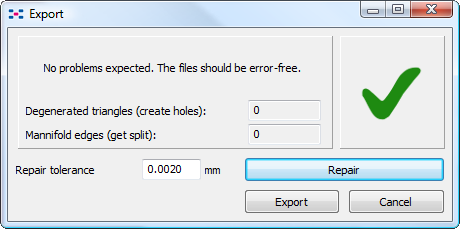
\includegraphics[keepaspectratio=true,width=0.75\textwidth]{working_with_models/netfabb_studio_export_part.png}
	\caption{Netfabb Studio: Part export.}
	\label{fig:netfabb_studio_export_part}
	\end{figure}
\end{itemize}
% paragraph netfabb_studio (end)

\paragraph{Netfabb Cloud Service} % (fold)
\label{par:netfabb_cloud_service}
Netfabb also hosts a web service where an STL file may be uploaded for it to be checked and repaired\footnote{http://cloud.netfabb.com/}.  

\begin{figure}[H]
\centering
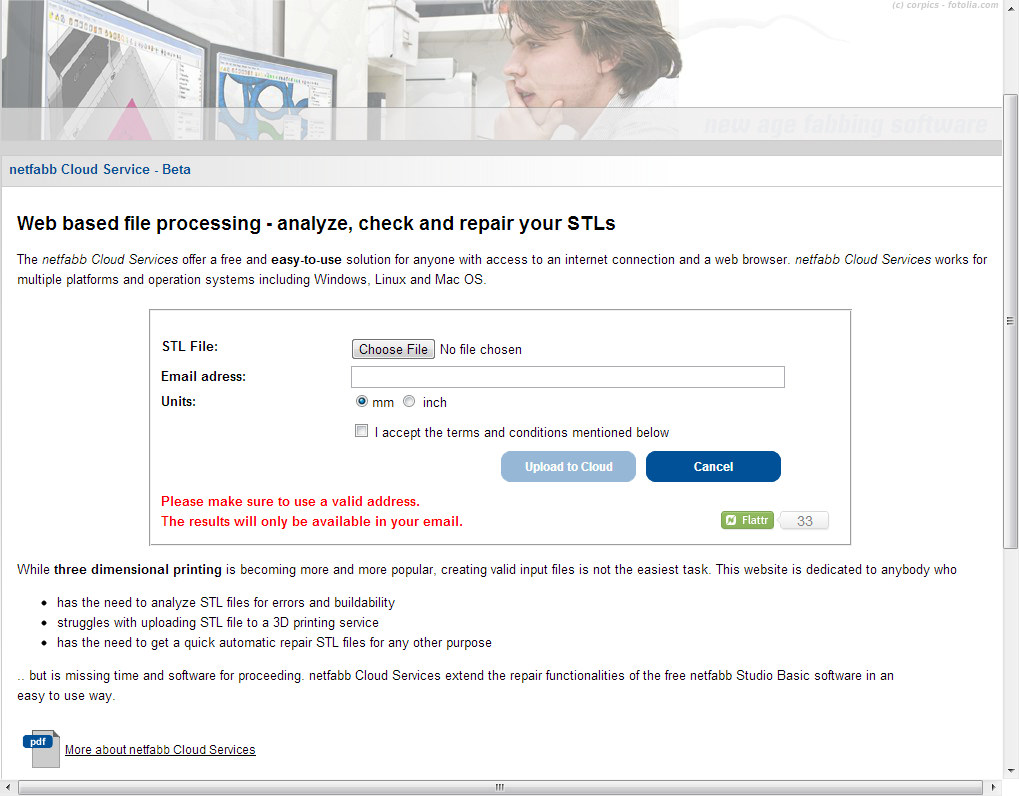
\includegraphics[keepaspectratio=true,width=0.75\textwidth]{working_with_models/netfabb_cloud_services.png}
\caption{Netfabb Cloud Services.}
\label{fig:netfabb_cloud_services}
\end{figure}

\begin{itemize}
	\item Navigate to http://cloud.netfabb.com
	\item Choose the STL file to upload using the button provided.
	\item An email address must be given to inform you when the service is finished.
	\item Choose whether metric or imperial measurements should be used.
	\item Read and accept the terms of service, and then click \texttt{Upload to Cloud}.
	\item Once the service has analysed and repaired the file an email is sent providing the download link to the repaired file.
\end{itemize}
}
%%% END CONFIGURATION TUNING %%%

\paragraph{FreeCAD} % (fold)
\label{par:freecad}
Freecad is a comprehensive, and free, CAD program which comes with a mesh module, in which repairs to degenerate models can be made.  the following steps outline how a problem model file can be analysed and repaired.

\begin{figure}[H]
\centering
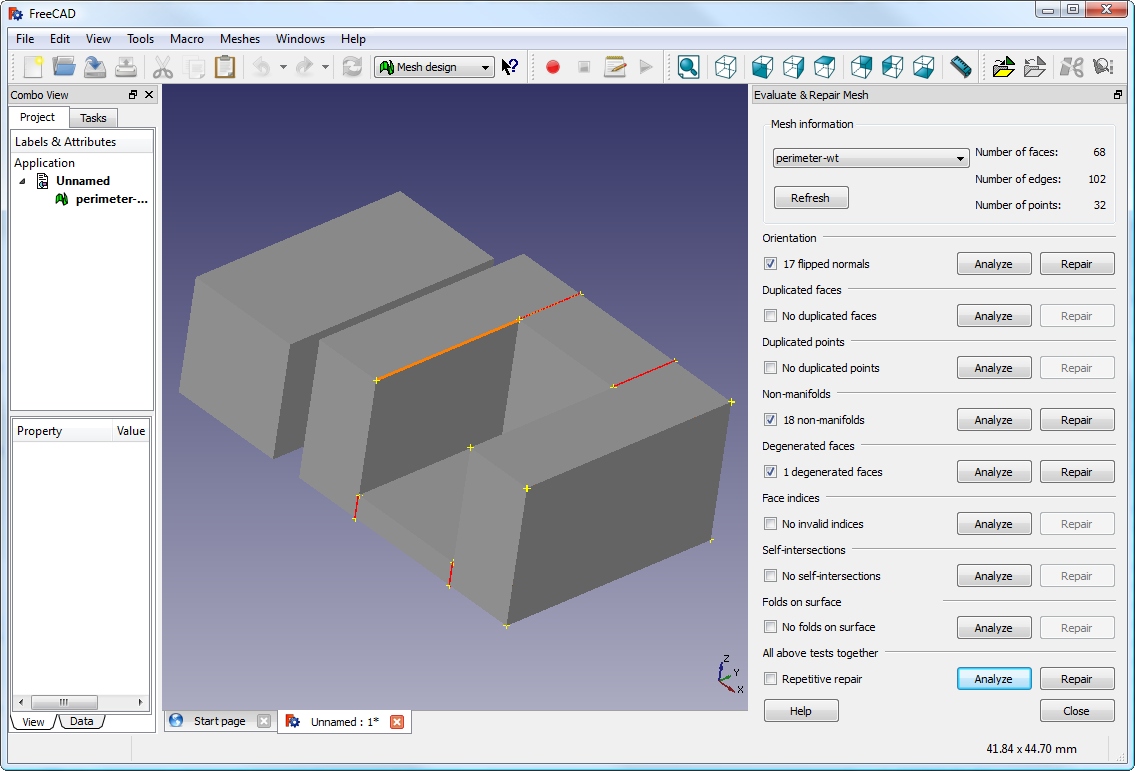
\includegraphics[keepaspectratio=true,width=0.75\textwidth]{working_with_models/freecad_part_repair.png}
\caption{FreeCAD part repair.}
\label{fig:freecad_part_repair}
\end{figure}

\begin{itemize}
	\item Start FreeCAD and from the start splash page choose \texttt{Working with Meshes}.  
	\item Load the model by dragging and dropping it onto the workspace or via the \texttt{File} menu.  A small message in the bottom left corner will indicate if the model appears to have problems.
	\item From the menu choose \texttt{Meshes->Analyze->Evaluate \& Repair mesh} to bring up the repair options dialog.
	\item From the options dialog choose the loaded mesh, then perform each analysis be clicking the \texttt{Analyze} button by each problem type, or select \texttt{Repetitive Repair} at the bottom to perform all checks.  If a corresponding problem is detected the \texttt{Repair} button becomes enabled.
	\item For each desired repair hit the \texttt{Repair} button.  
	\item It is important to review the effect the repair script has made to the model.  It may be the case that the script damages the file, rather than repair, for example by removing important triangles.
	\item Export the repaired model via the \texttt{Export} menu option or context menu.
\end{itemize}
% paragraph freecad (end)

% subsection cleaning_stls (end)